\appendix
\section{Prozessdiagramme}

\begin{figure}[H]
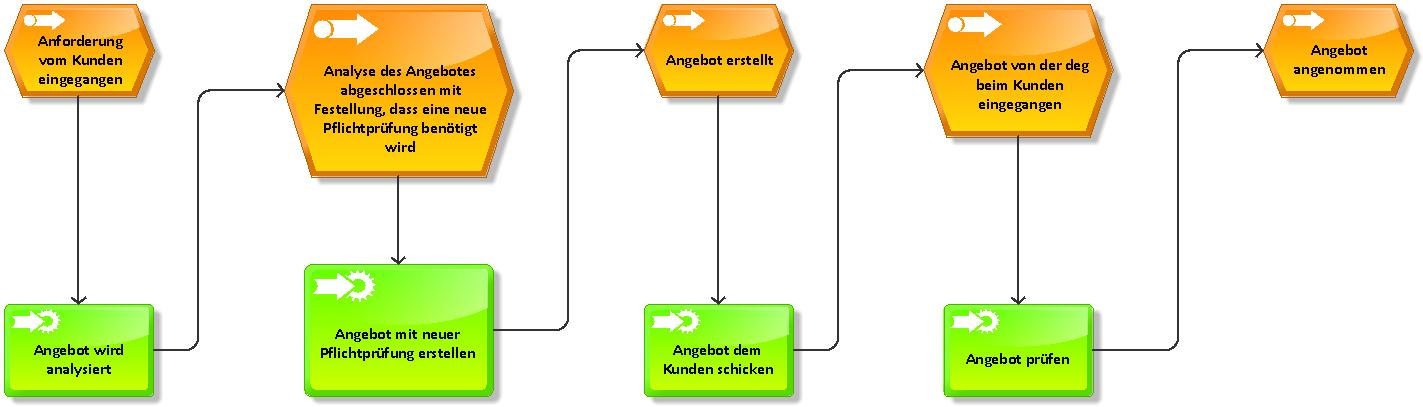
\includegraphics[scale=0.3]{anforderungundanalyse.jpeg}
\caption{Teilprozess:
Anforderung und Analyse}\label{Anforderung und Analyse}
\end{figure}

\begin{figure}[H]
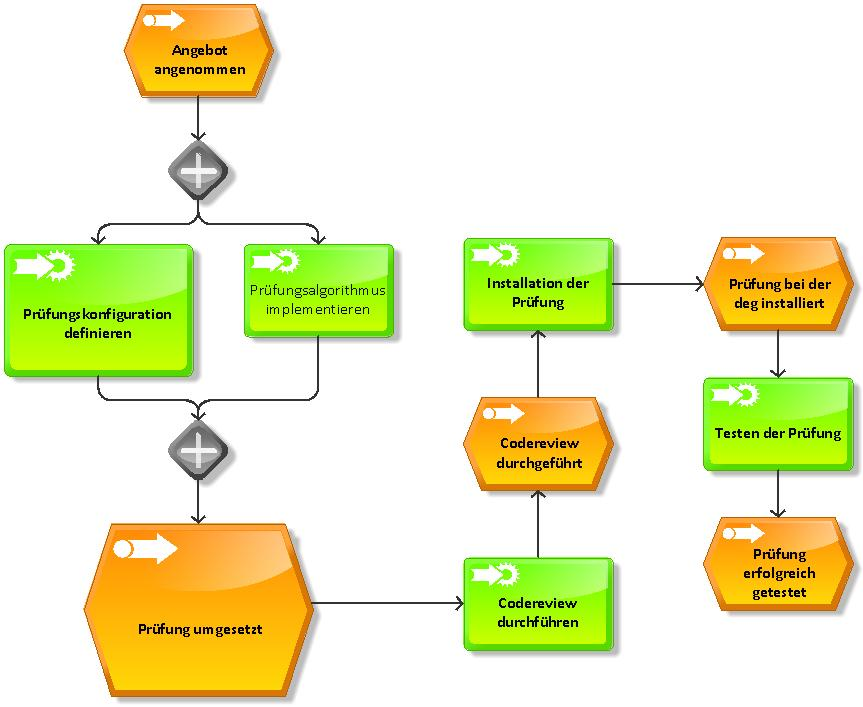
\includegraphics[scale=0.5]{umsetzung.jpeg}
\caption{Teilprozess:
Umsetzung}\label{Umsetzung}
\end{figure}


\begin{figure}[H]
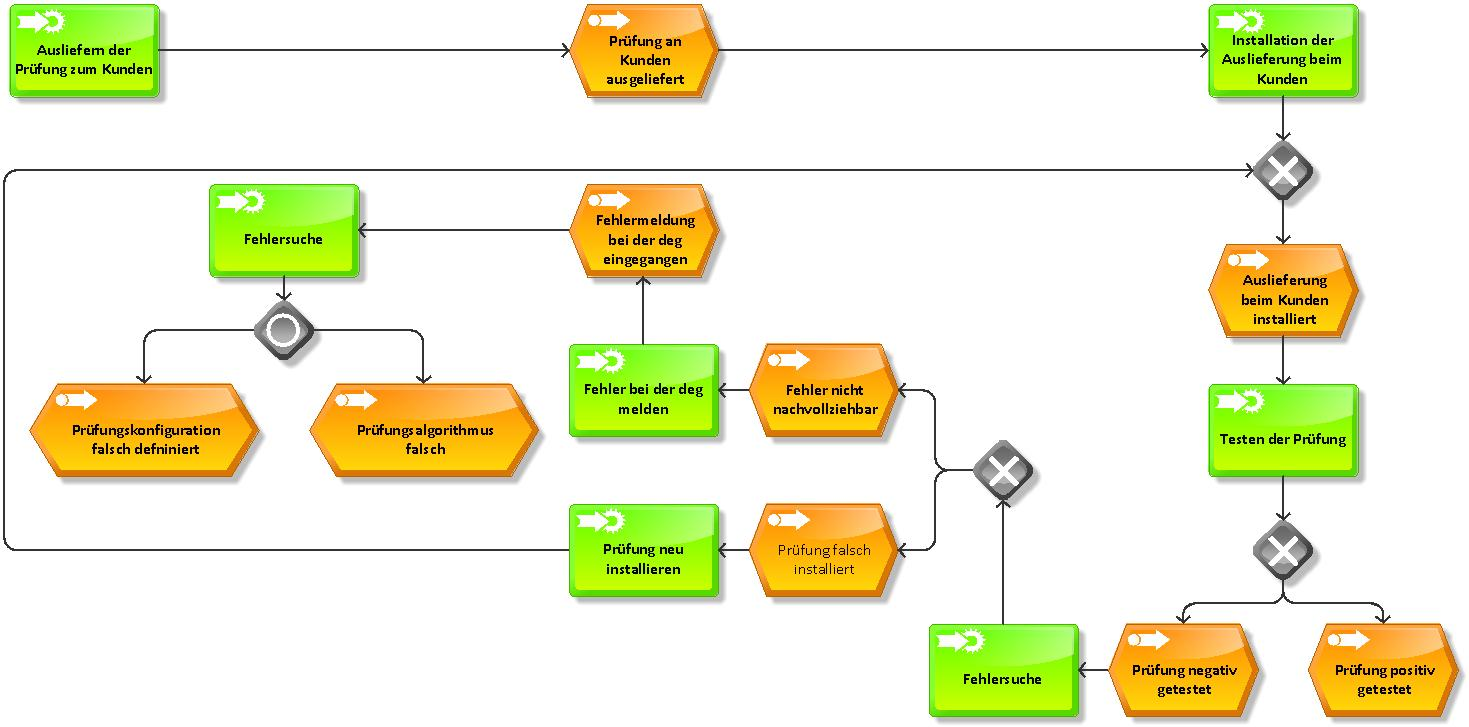
\includegraphics[scale=0.3]{auslieferung.jpeg}
\caption{Teilprozess:
Auslieferung}\label{Auslierferung}
\end{figure}


\section{Inhalt des beiliegenden Datentr�gers}\label{an}
\begin{itemize}
  \item  []\textbf{Grammatik f�r die Syntax der
  Konfigurationsdateien:}
  \newline Implementierung/xtext/de.deg.eler.ft.vp/src/de/deg/eler\\/ft/vp/Dsl.xtext
  
  \item []\textbf{Validator-Klasse f�r die Konfigurationsdateien:}\\
  Implementierung/xtext/de.deg.eler.ft.vp/src/de/deg/eler\\/ft/vp/validation/DslValidator.xtend
  
  \item []\textbf{Eclipse Distribution:}\\
  Eclipse/eclipse.exe
  
  \item []\textbf{Quellen in PDF-Form:}\\
  PDFs/
  
  \item []\textbf{Internetquellen:}\\
  Internet/
\end{itemize}
